\documentclass[12pt,a4paper]{article}
\usepackage[utf8]{inputenc}
%加這個就可以設定字體
\usepackage{fontspec}
%使用xeCJK,其他的還有CJK或是xCJK
\usepackage{xeCJK}
\usepackage{enumerate}
%設定英文字型,不設的話就會使用預設的字型
\usepackage{hyperref}
\usepackage{graphicx}
\usepackage{geometry}
\geometry{a4paper,scale=0.8}
\setmainfont{Times New Roman}
\usepackage{listings}
\usepackage{amsfonts} %數學簍空的英文字
\lstset{language=python}
%設定中英文的字型
%字型的設定可以使用系統內的字型,而不用像以前一樣另外安裝
\setCJKmainfont{標楷體}
%以下是新增的自定义格式更改
\usepackage[]{caption2} %新增调用的宏包
\renewcommand{\figurename}{fig} %重定义编号前缀词
%中文自動換行
\XeTeXlinebreaklocale "zh"

%文字的彈性間距
\XeTeXlinebreakskip = 0pt plus 1pt

%設定段落之間的距離
\setlength{\parskip}{0.3cm}
\title{Deep Reinforcement Learning Pong game }
\author{虎尾科技大學\\40723115\\ 林于哲}
\date{January 16 2021}

\begin{document}
\maketitle
\tableofcontents



\section{openAI Gym}
Gym 是用於開發和比較強化學習算法的工具包,他不對agent的結構做任何假設,並且與任何數據計算庫兼容,而可以用來制定強化學習的算法。這個環境具有共享的介面,使我們能用來編寫常規算法,也就能教導agents如何步行到玩遊戲。\\[6pt]


\section{Pong}
取自 1977年發行的一款家用遊戲機ATARI 2600中的遊戲,內建於Gym,這是一個橫向的乒乓遊戲,左方是遊玩者,右邊是馬可夫決策的特例,每個邊緣都會給予reward(figue1),目標就是計算再任意階段動作最佳路徑,已獲得rewardd最大值。
\section{Abstract}
I'd like to walk you through Policy Gradients (PG), our favorite default choice for attacking RL problems at the moment. If you’re from outside of RL you might be curious why I’m not presenting DQN instead, which is an alternative and better-known RL algorithm, widely popularized by the ATARI game playing paper. It turns out that Q-Learning is not a great algorithm (you could say that DQN is so 2013 . In fact most people prefer to use Policy Gradients, including the authors of the original DQN paper who have shown Policy Gradients to work better than Q Learning when tuned well. PG is preferred because it is end-to-end: there's an explicit policy and a principled approach that directly optimizes the expected reward. Anyway, as a running example we'll learn to play an ATARI game (Pong!) with PG, from scratch, from pixels, with a deep neural network, and the whole thing is 130 lines of Python only using numpy as a dependency (Gist link). Lets get to it.

\section{Pong from pixels}
Left: The game of Pong. Right: Pong is a special case of a Markov Decision Process (MDP): A graph where each node is a particular game state and each edge is a possible (in general probabilistic) transition. Each edge also gives a reward, and the goal is to compute the optimal way of acting in any state to maximize rewards.\\ 
The game of Pong is an excellent example of a simple RL task. In the ATARI 2600 version we’ll use you play as one of the paddles (the other is controlled by a decent AI) and you have to bounce the ball past the other player (I don’t really have to explain Pong, right?). On the low level the game works as follows: we receive an image frame (a 210x160x3 byte array (integers from 0 to 255 giving pixel values)) and we get to decide if we want to move the paddle UP or DOWN (i.e. a binary choice). After every single choice the game simulator executes the action and gives us a reward: Either a +1 reward if the ball went past the opponent, a -1 reward if we missed the ball, or 0 otherwise. And of course, our goal is to move the paddle so that we get lots of reward.\\


\section{Deep Reinforcement Learning}

\begin{figure}[hbt!]
\begin{center}
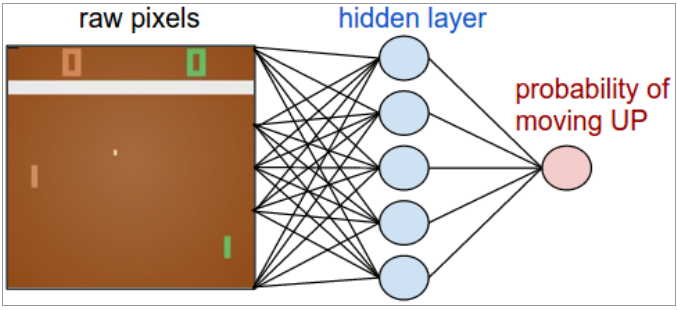
\includegraphics[scale=0.74]{ network}
\caption{Our network is a 2-layer fully-connected net. }%from: \href{file:///H:/201906_fall/data/tmp/project2020-1/downloads/reinforcement_learning/2018_Book_ReinforcementLearning.pdf}{All the faces of Reinforcement Learning}
\end{center}
\end{figure}\textbf{}

we're going to define a policy network that implements our player (or “agent”). This network will take the state of the game and decide what we should do (move UP or DOWN). As our favorite simple block of compute we'll use a 2-layer neural network that takes the raw image pixels (100,800 numbers total (210*160*3)), and produces a single number indicating the probability of going UP. Note that it is standard to use a stochastic policy, meaning that we only produce a probability of moving UP. Every iteration we will sample from this distribution (i.e. toss a biased coin) to get the actual move. The reason for this will become more clear once we talk about training.\\


\section{Supervised Learning}
\begin{figure}[hbt!]
\begin{center}
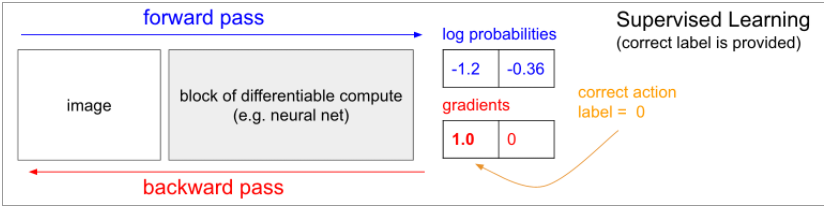
\includegraphics[scale=0.74]{supervising learning}
\caption{supervising learning }%from: \href{file:///H:/201906_fall/data/tmp/project2020-1/downloads/reinforcement_learning/2018_Book_ReinforcementLearning.pdf}{All the faces of Reinforcement Learning}
\end{center}
\end{figure}
\textbf{}
Before we dive into the Policy Gradients solution I'd like to remind you briefly about supervised learning because, as we'll see, RL is very similar. Refer to the diagram below. In ordinary supervised learning we would feed an image to the network and get some probabilities, e.g. for two classes UP and DOWN. I'm showing log probabilities (-1.2, -0.36) for UP and DOWN instead of the raw probabilities (30 persent and 70 persent in this case) because we always optimize the log probability of the correct label (this makes math nicer, and is equivalent to optimizing the raw probability because log is monotonic). Now, in supervised learning we would have access to a label. For example, we might be told that the correct thing to do right now is to go UP (label 0). In an implementation we would enter gradient of 1.0 on the log probability of UP and run backprop to compute the gradient vector $Wlogp(y=UP|x)$. This gradient would tell us how we should change every one of our million parameters to make the network slightly more likely to predict UP. For example, one of the million parameters in the network might have a gradient of -2.1, which means that if we were to increase that parameter by a small positive amount (e.g. 0.001), the log probability of UP would decrease by 2.1 * 0.001 (decrease due to the negative sign). If we then did a parameter update then, our network would now be slightly more likely to predict UP when it sees a very similar image in the future.\\

\section{Log Derivative Trick}
機器學習涉及操縱機率。這個機率通常包含normalised-probabilities或 log-probabilities。能加強解決現代機器學習問題的關鍵點,是能夠巧妙的在這兩種型式間交替使用,而對數導數技巧就能夠幫助我們做到這點,也就是運用對數導數的性質。\\
\section{Score Functions}
對數導數技巧的應用規則是基於參數$\theta$梯度的對數函數$p(x:\theta)$,如下:\\
$$\nabla_\theta logp(x:\theta)=\frac{\nabla_\theta p(x:\theta)}{p(x:\theta)}$$\\
$p(x:\theta)$是likelihood ; function參數$\theta$的函數,它提供隨機變量x的概率。在此特例中,$\nabla_\theta logp(x:\theta)$被稱為Score Function,而上述方程式右邊為score ratio(得分比)。\\[6pt]

\begin{mini}{The score function has a number of useful properties:}\end{mini}
\begin{itemize}
\item The central computation for maximum likelihood estimation. Maximum likelihood is one of the dominant learning principles used in machine learning, used in generalised linear regression, deep learning, kernel machines, dimensionality reduction, and tensor decompositions, amongst many others, and the score appears in all these problems. 
\end{itemize}
\begin{itemize}
\item The expected value of the score is zero. Our first use of the log-derivative trick will be to show this.\\
$$\mathbb{E}_{p(x; \theta)}[\nabla_\theta \log p(\mathbf{x}; \theta)] =\mathbb{E}_{p(x; \theta)}\left[\frac{\nabla_\theta p(\mathbf {x}; \theta)}{p(\mathbf{x}; \theta)} \right]$$
$$= \int p(\mathbf {x}; \theta) \frac{\nabla_\theta p(\mathbf {x}; \theta)}{p(\mathbf{x}; \theta)} dx= \nabla_\theta \int p(\mathbf{x}; \theta) dx=\nabla_\theta 1 = 0$$\\
In the first line we applied the log derivative trick and in the second line we exchanged the order of differentiation and integration. This identity is the type of probabilistic flexibility we seek: it allows us to subtract any term from the score that has zero expectation, and this modification will leave the expected score unaffected (see control variates later).
\end{itemize}
\begin{itemize}
\item The variance of the score is the Fisher information and is used to determine the Cramer-Rao lower bound.\\
$$\mathbb{V}[\nabla_\theta \log p(\mathbf{x}; \theta)] = \mathcal{I}(\theta) =\mathbb{E}_{p(x; \theta)}[\nabla_\theta \log p(\mathbf{x}; \theta)\nabla_\theta \log p(\mathbf{x}; \theta)^\top]$$\\
We can now leap in a single bound from gradients of a log-probability to gradients of a probability, and back. But the villain of today's post is the troublesome expectation-gradient of Trick 4, re-emerged. We can use our new-found power—the score function—to develop yet another clever estimator for this class of problems.
\end{itemize}
\section{Score Function Estimators}
Our problem is to compute the gradient of an expectation of a function f:\\
$$\nabla_\theta \mathbb{E}_{p(z;\theta)}[f(z)] =\nabla_\theta \int p(z; \theta)f(z) dz$$\\

This is a recurring task in machine learning, needed for posterior computation in variational inference, value function and policy learning in reinforcement learning, derivative pricing in computational finance, and inventory control in operations research, amongst many others.

This gradient is difficult to compute because the integral is typically unknown and the parameters θ, with respect to which we are computing the gradient, are of the distribution p(z;θ). Furthermore, we might want to compute this gradient when the function f is not differentiable. Using the log derivative trick and the properties of the score function, we can compute this gradient in a more amenable way:\\
$$\nabla_\theta \mathbb{E}_{p(z;\theta)}[f(z)] = \mathbb{E}_{p(z;\theta)}[f(z)\nabla_\theta \log p(z;\theta)]$$\\
This is a recurring task in machine learning, needed for posterior computation in variational inference, value function and policy learning in reinforcement learning, derivative pricing in computational finance, and inventory control in operations research, amongst many others.

This gradient is difficult to compute because the integral is typically unknown and the parameters θ, with respect to which we are computing the gradient, are of the distribution p(z;θ). Furthermore, we might want to compute this gradient when the function f is not differentiable. Using the log derivative trick and the properties of the score function, we can compute this gradient in a more amenable way:\\
$$\nabla_\theta \mathbb{E}_{p(z;\theta)}[f(z)] = \mathbb{E}_{p(z;\theta)}[f(z)\nabla_\theta \log p(z;\theta)]$$\\
\begin{figure}[hbt!]
\begin{center}
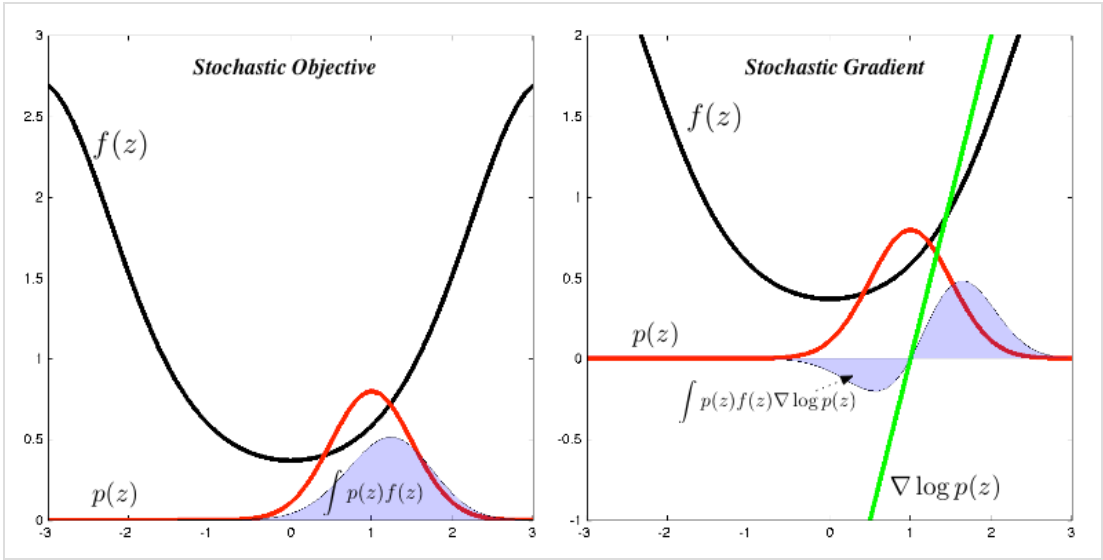
\includegraphics[scale=0.6]{gradient change}
\caption{gradient change}%from: \href{file:///H:/201906_fall/data/tmp/project2020-1/downloads/reinforcement_learning/2018_Book_ReinforcementLearning.pdf}{All the faces of Reinforcement Learning}
\end{center}
\end{figure}
Let's derive this expression and explore the implications of it for our optimisation problem. To do this, we are will use one other ubiquitous trick, a probabilistic identity trick, where we multiply our expressions by 1—a one formed by the division of a probability density by itself.  Combining the identity trick with the log-derivative trick, we obtain a score function estimator for the gradient:\\
$$\nabla_\theta \mathbb{E}_{p(z;\theta)}[f(z)]=\int\nabla_\theta p(z;\theta)f(z) dz$$\\[6pt]
$$= \int \frac{p(z;\theta)}{p(z;\theta)}\nabla_\theta p(z;\theta)f(z) dz$$\\[6pt]
$$=\int p(z;\theta)\nabla_\theta \log p(z;\theta)f(z) dz = \mathbb{E}_{p(z;\theta)}[f(z)\nabla_\theta \log p(z;\theta)]$$\\[6pt]
$$=\int p(z;\theta)\nabla_\theta \log p(z;\theta)f(z) dz = \mathbb{E}_{p(z;\theta)}[f(z)\nabla_\theta \log p(z;\theta)]$$\\[6pt]
$$\approx \frac{1}{S} \sum_{s=1}^{S}f(z^{(s)})\nabla_\theta \log p(z^{(s)};\theta) \quad z^{(s)}\sim p(z)$$\\[6pt]
A lot has happened in these four lines. In the first line we exchanged the derivative and the integral. In the second line, we applied our probabilistic identity trick, which allowed us to form the score ratio. Using the log-derivative trick, we then replaced this ratio with the gradient of the log-probability in the third line. This gives us our desired stochastic estimator in the fourth line, which we computed by Monte Carlo by first drawing samples from p(z) and then computing the weighted gradient term.\\

To put this in English, we have some distribution $p(x;\theta)$ (I used shorthand $p(x)$ to reduce clutter) that we can sample from (e.g. this could be a gaussian). For each sample we can also evaluate the score function f which takes the sample and gives us some scalar-valued score. This equation is telling us how we should shift the distribution (through its parameters θ) if we wanted its samples to achieve higher scores, as judged by f. In particular, it says that look: draw some samples x, evaluate their scores f(x), and for each x also evaluate the second term $\nabla_\theta logp(x;θ)$. What is this second term? It’s a vector - the gradient that’s giving us the direction in the parameter space that would lead to increase of the probability assigned to an x. In other words if we were to nudge θ in the direction of $\nabla_\theta logp(x;θ)$ we would see the new probability assigned to some x slightly increase. If you look back at the formula, it’s telling us that we should take this direction and multiply onto it the scalar-valued score $f(x)$. This will make it so that samples that have a higher score will “tug” on the probability density stronger than the samples that have lower score, so if we were to do an update based on several samples from p the probability density would shift around in the direction of higher scores, making highly-scoring samples more likely.
\begin{figure}[hbt!]
\begin{center}
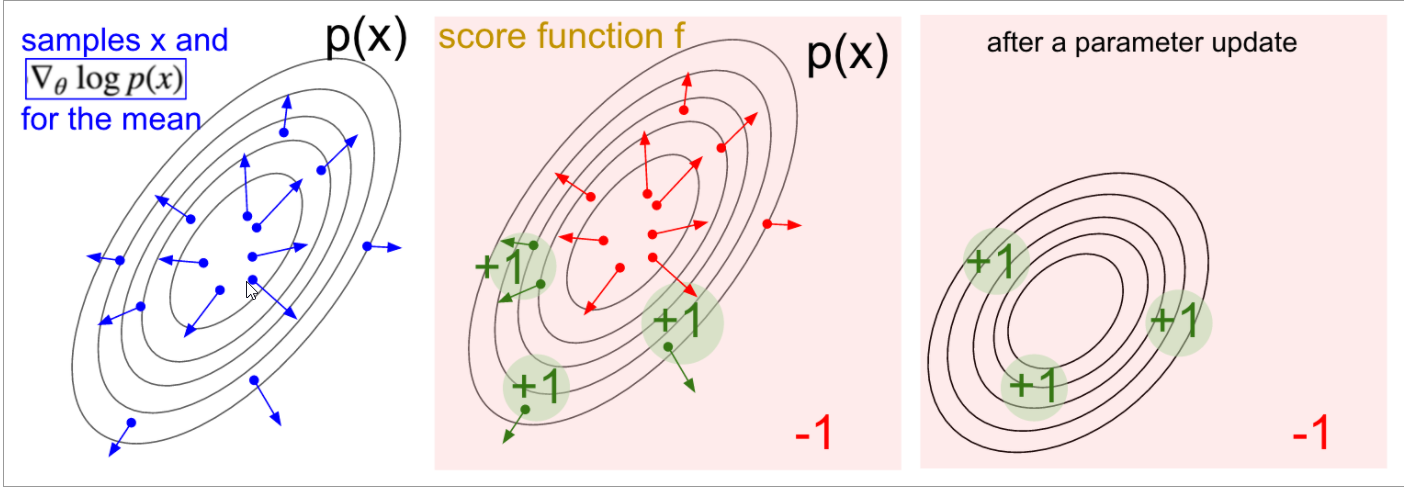
\includegraphics[scale=0.4]{figure}
%\caption{gradient change}%from: \href{file:///H:/201906_fall/data/tmp/project2020-1/downloads/reinforcement_learning/2018_Book_ReinforcementLearning.pdf}{All the faces of Reinforcement Learning}
\end{center}
\end{figure}
A visualization of the score function gradient estimator. Left: A gaussian distribution and a few samples from it (blue dots). On each blue dot we also plot the gradient of the log probability with respect to the gaussian's mean parameter. The arrow indicates the direction in which the mean of the distribution should be nudged to increase the probability of that sample. Middle: Overlay of some score function giving -1 everywhere except +1 in some small regions (note this can be an arbitrary and not necessarily differentiable scalar-valued function). The arrows are now color coded because due to the multiplication in the update we are going to average up all the green arrows, and the negative of the red arrows. Right: after parameter update, the green arrows and the reversed red arrows nudge us to left and towards the bottom. Samples from this distribution will now have a higher expected score, as desired.\\

\end{document}  